
\chapter{Operad of Welded Braids} 

We want to prove that welded braids form an operad, i.e. we want to see if we can define a composition operation \( \circ_i \) on the set of braids \( wB \) which is a natural extension of the composition of classical braids.
Thankfully in this case the same definition works as before, where we define an interval around the \( i \)th strand at each height and replace into our braid for each height. 

\section{The Composition of Welded Braids} \label{sec:wb_composition}

Consider welded braids \( A \in wB_n \) and \( B \in wB_m \) and \( i \in [n] \).
We define \( A \circ_i B \) by considering the classical braid definition of the \( \circ_i \) operator and performing it analogously on welded braids. 

\begin{Theorem}
    For welded braids \( A \in wB_n \) and \( B \in wB_m\) and index \( i \in [n] \). 
    \( A \circ_i B \) isn't well defined.
\end{Theorem}

\begin{proof} \label{pr:counter}

We prove by counter example. 
Let \( A = \sigma_1 \in wB_2 \) and \( B = s_1 \in wB_2 \), and consider \( A \circ_1 B \). 

\begin{figure}[H]
    \centering
    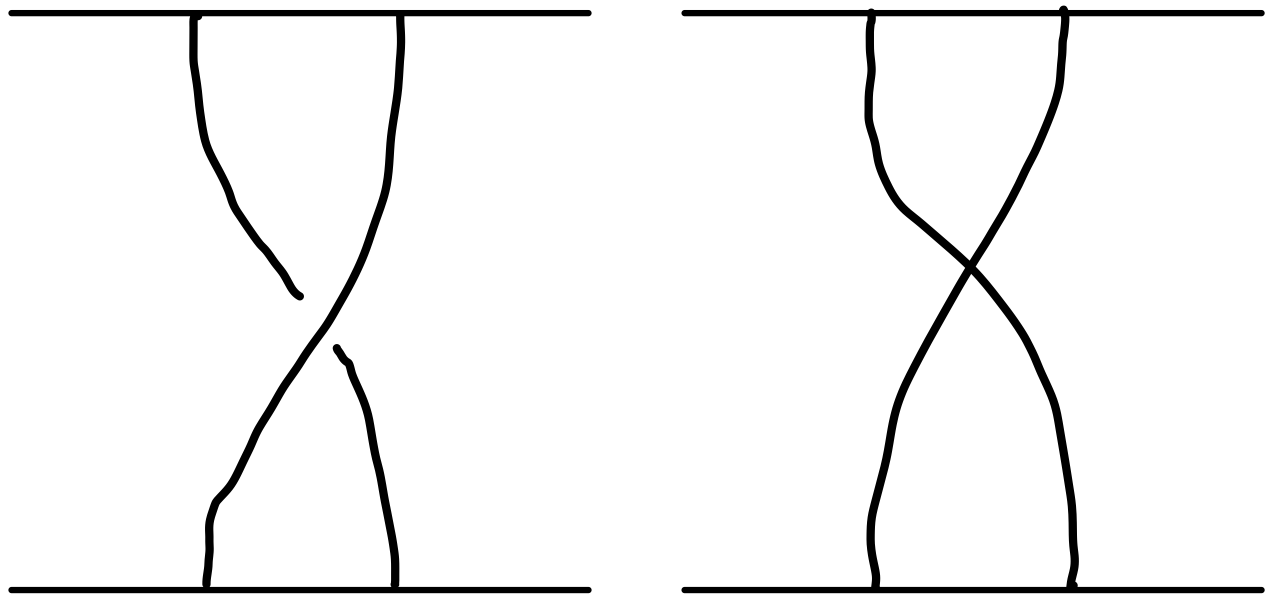
\includegraphics[width=0.8\textwidth]{images/welded_braids/3_welded_proof_values.png}
    \caption{\( A \) (left) and \( B \) (right)}
\end{figure}

Because there is a single crossing for each braid this implies that there exists a single point at height \( t = \frac{1}{2} \) where the crossings occur. 

Therefore we will arbitrarily consider which crossing occurs first by considering the cases where the crossings originating from \( A \) occur first, or the crossing originating from \( B \) occurs first. 
This is shown via the diagrams

% Picture of the braids
\begin{figure}[H]
    \centering
    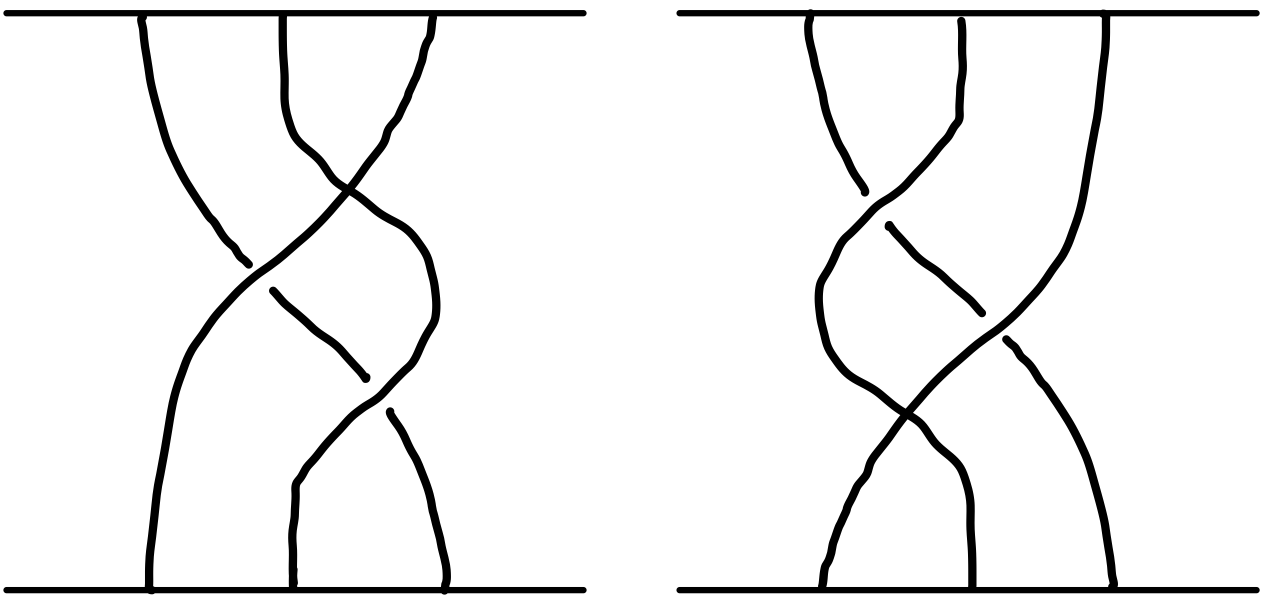
\includegraphics[width=0.8\textwidth]{images/welded_braids/4_welded_proof.png}
    \caption{Two outputs of \( A \circ_1 B\) depending on if the crossings in \( A \) occur first (left), or the crossings in \( B \) occur first (right).}
    \label{fig:UC}
\end{figure}

Which can be represented by
\[
A \circ_1 B =
\begin{cases}
\sigma_2 \sigma_1 s_2 &\text{If A occurs first} \\
s_1 \sigma_2 \sigma_1 &\text{If B occurs first} \\
\end{cases}
\]
However this is the \emph{UC} relation, which was shown to explicitly not to be equivalent in \cref{ex:UC}.
And thus the \( \circ_i \) operation we defined is not well defined and therefore doesn't form an operad.
\end{proof}

\section{The Non-Canonical Operad of Welded Braids}

We shall now consider how we might fix the problems presented in \cref{sec:wb_composition}.

We can consider a handful of decisions to make the composition operation well defined, however we're going to consider the arbitrary decision where if there is height in which two crossings occur simultaneously, then we arbitrarily decide to perform the crossing of the input braid first. 
E.g. for counter-example in \cref{pr:counter} this would result in \( A \circ_1 B = s_1\sigma_2\sigma_1 \), implying that this composition operation is well defined. 

\begin{Theorem}
    Welded Braids form a non-canonical Operad under this composition operation. 
\end{Theorem}

\begin{proof}
Let's consider the category of welded braids \( \WB \), where welded braids are our objects \( \Ob(\WB) := wB \) and the permutations of the names of the strands are our morphisms. 

We consider the functor \( \WB \map{\Sn}{\WB} \), where \( \WB(n) = wB_n \) for \( n \in \N \). 
We then consider a composition operation \( \circ_i \) defined as mentioned above, and we show that the associativity rules hold.

For \( n, m, k \in \N \), indices \( i_1, i_2 \in [n] \) where \( i_1 \neq i_2 \), and braids \( A \in \WB(n), B \in \WB(m), \) and \( C \in \WB(k) \)
\[ (A \circ_{i_1} B) \circ_{i_2} C = (A \circ_{i_2} C) \circ_{i_1} A \]
This is because inputting into two different strands in a different order don't effect each other, as the composition is a property of the single strand only. 
And for indices \( i \in [n] \) and \( j \in [m] \)
\[ (A \circ_i B) \circ_j C = A \circ_i (B \circ_j C) \]
This is because composition is an operation on a single braid, and can be performed in place inside another braid. 

Finally we consider the unit morphism \( e \) as the single braid \( 1 \in \WB(1) \). 
Evidently, replacing a strand in a braid with a strand will result in the same braid. 
And replacing the singular strand in \( 1 \) with a braid will result in the braid. 
Thus for a braid \( B \in WB(n) \) and \( i \in [n] \)
\[ B = B \circ_i e = e \circ_i B \]
And therefore \( \{ \WB(n) \}_{n \ge 0} \) forms a non-canonical operad. 
\end{proof}

\begin{Exercise}
    Consider \( A = s_1 \sigma_2 s_2 \sigma_1^{-1} \in \WB(3) \) and \( B = \sigma_1 s_2\sigma_3^{-1} \in \WB(4) \). 
    In the operad \( \WB \), compute \( A \circ_1 B \), \( A \circ_3 B \), and \( B \circ_2 A \). 
\end{Exercise}

% \section{Further Composition}

% Any composition we define will be non-canonical in nature, and therefore this is a dead-end.
% We could define other composition operations, however no new insights would be gained. 
% However we can consider many questions if we break symmetry. 
% Instead of only inputting welded braids into welded braids, we consider inputting usual braids into welded braids?
% Or define a 


% Where evidently for any braid \( B \), replacing a strand with a single strand always results in the same braid \( B \) and similarly, replacing the single strand of \( \bullet \) with the whole braid \( B \) results in the braid \( B \).
% And therefore \( B =  B \circ_i \bullet = \bullet \circ_1 B \). 
% We first need to create our \( \Sn \)-Module by determining a symmetric monoidal category, where our objects are welded braids. 
% It's of note that we're considering the specialisation of the definition of an operad, because the only information that a given braid within our operad has is the number of strands it contains. 

% Let \( \WB \) be the category where \( wB := \Ob(\WB) \), our morphisms consist of permuting the names strands of the braids, and our product operation \( \otimes \) is the cartesian product.
% Let \( n \in \N \) and define our \( \Sn \)-module such that.
% \begin{align*} 
%     \WB : \Sn   &\to \WB \\
%     [n] \in \Sn &\mapsto wB_n \in \Ob(\WB)
% \end{align*}
% Where a given permutation of \( n \) objects in \( \Sn \) is mapped to a function which permutes the names of any braid in \( wB_n \) by that permutation. 

% We then consider our composition operation, however this axiom is satisfied by seeing for welded braids \( A \in \WB(n_A) \), \( B \in \WB(n_B) \), and \( C \in \WB(n_C) \) and \( i_1, i_2 \in [n_A] \) where \( i_1 \neq i_2 \) we know.
% \[ (A \circ_{i_1} B) \circ_{i_2} C = (A \circ_{i_2} C) \circ_{i_1} B \]
% This is because inputting into two different strands in a different order don't effect each other, as the replacement is a property of the single strand only. 
% And for \( i \in [n_A] \) and \( j \in [n_B] \) we know
% \[ (A \circ_i B) \circ_j C = A \circ_i (B \circ_j C) \]
% This is because irrespective of the 
% And thus the associativity diagrams for operads commute. 

% Finally we consider the unit morphism \( e : \mathbb{1} \to \WB(1) \), where our identity for the cartesian product \( \mathbb{1} \) is the empty braid in \( wB_0 \), i.e. no strands, and this is mapped to the single element in \( \bullet \in wB_1 \), i.e. 1 singular strand. 
% Where evidently for any braid \( B \), replacing a strand with a single strand always results in the same braid \( B \) and similarly, replacing the single strand of \( \bullet \) with the whole braid \( B \) results in the braid \( B \).
% And therefore \( B =  B \circ_i \bullet = \bullet \circ_1 B \). 